\RequirePackage{lineno}
\documentclass[conference]{IEEEtran}
%\documentclass[draft, onecolumn]{IEEEtran}
% correct bad hyphenation here
\hyphenation{op-tical net-works semi-conduc-tor}

% =============+s\\==================================================
%\usepackage{subfigure, graphicx, booktabs}
%\usepackage{algpseudocode, algorithmicx, algorithm}
\usepackage{amsmath, amsthm, listings, booktabs}

%Code environment
\newcommand{\code}[1]{{\tt#1}}
\newcommand{\todo}[1]{\textbf{TODO: #1}}
\newcommand\inputsrc[1]{{\tt \lstinputlisting[]{source/#1} }}
\newcommand{\reffig}[1]{Fig.~\ref{fig:#1}}
\newcommand{\reftable}[1]{Table~\ref{tbl:#1}}
\long\def\comment#1{}

\def\ssp{\def\baselinestretch{0.99}\large\normalsize}

%\addtolength{\columnsep}{-3mm}

% setup listing parameters
%\lstloadlanguages{c++,c}
\lstset{language=c++,basicstyle=\scriptsize}
\lstset{numbers=left,numberstyle=\tiny,stepnumber=1}
%%\lstset{labelstep=1}
%\lstset{stringspaces=false}
\lstset{stringstyle=\tt}
%\lstset{singlecomment={/*}{*/}}
%\lstset{commentline=/*}
\lstset{commentstyle=\it}
\lstset{morekeywords={pragma, par, seq, par_tail, _tail, reduce, omp, parallel}} 
%%\lstset{indent=6mm}
\lstset{xleftmargin=6mm}

% *** GRAPHICS RELATED PACKAGES ***
%
\ifCLASSINFOpdf
   \usepackage[pdftex]{graphicx}
  % declare the path(s) where your graphic files are
   \graphicspath{{../pdf/}{../jpeg/}}
  % and their extensions so you won't have to specify these with
  % every instance of \includegraphics
   \DeclareGraphicsExtensions{.pdf,.jpeg,.png}
   \DeclareGraphicsRule{*}{mps}{*}{}
\else
  % or other class option (dvipsone, dvipdf, if not using dvips). graphicx
  % will default to the driver specified in the system graphics.cfg if no
  % driver is specified.
   \usepackage[dvips]{graphicx}
  % declare the path(s) where your graphic files are
   \graphicspath{{./}}
  % and their extensions so you won't have to specify these with
  % every instance of \includegraphics
   \DeclareGraphicsExtensions{.png, .pdf, .eps}
\fi

% ===============================================================
\newtheorem{theorem}{Theorem}[section]
\newtheorem{conjecture}[theorem]{Conjecture}
\newtheorem{corollary}[theorem]{Corollary}
\newtheorem{proposition}[theorem]{Proposition}
\newtheorem{lemma}[theorem]{Lemma}
%\newdef{definition}[theorem]{Definition}
%\newdef{remark}[theorem]{Remark}


\begin{document}
\title{A Template Metaprogramming Approach to Support Parallel
  Programs for Multicores}


% author names and affiliations
% use a multiple column layout for up to three different
% affiliations
\author{
\IEEEauthorblockN{Xin Liu, Minyi Guo, Daqiang Zhang, Jingyu Zhou, Yao Shen}
\IEEEauthorblockA{Department of Computer Science\\
Shanghai Jiao Tong University\\
No. 800, Dongchuan Road, Shanghai, P.R.China\\
navyliu@sjtu.edu.cn}
}
%\{guo-my\}@cs.sjtu.edu.cn,
%\{zhangdq\}@sjtu.edu.cn, \{zhou-jy, shen\_yao\}@cs.sjtu.edu.cn
% make the title area
\maketitle


\begin{abstract}
In advent of multicore era, plain C/C++ programming languages can not
fully reflect computer architectures. Source-to-source
transformations help tailor programs close to contemporary
hardwares. In this paper, we propose template-based approach to perform 
transformations for programs with rich static information.
We present C++ template metaprogramming techniques to conduct
parallelization for specific
multicores. Parallel patterns and executions are provided in the form of
template classes and oraganized as library. We implement a prototype
template library -- Libvina, to demonstrate the idea. It enables
programmers to utilize new architectural
features and add parallelization strategies by extending template library. 
Finally, we evaluate our template library on
commodity x86 and GPU platforms by a variety of typical procedures
in multimedia and scientific fields. In experiments, we show that our
approach is flexible to support multiple parallel models and capable
of transforming sequential codes to parallel equivalences according to
specific multicore architectures. Moreover, the cost of programmability using our
approach to adapt to more than one multicore is manageable.
\end{abstract}

% For peerreview papers, this IEEEtran command inserts a page break and
% creates the second title. It will be ignored for other modes.
\IEEEpeerreviewmaketitle


%\section{Related work}\label{sec:related}
%\begin{figure}
%  % Requires \usepackage{graphicx}
%  \centering
%  \includegraphics[width=0.8\linewidth]{../fig/motivation}
%  \caption{CFSF Motivation}\label{fig:motivation}
%  \label{fig:algorithm}
%\end{figure}
\section{Introduction}\label{sec:Intro}
%multicore problem
Modern computer architectures rely on parallelism and memory
hierarchy to improve performance. Both duplicated processors and
elaborated storage-on-chip require programmers to be aware of underlying
machines when they write programs. Even worse,
multicore technologies have brought various architectural features for
different implementations. Thus, it is challenging to develop
efficient applications which can take advantage of various multicores.

%need new programming model
In essence, it is because plain C/C++ programming language
can not reflect contemporary architectures. Traditionally, programmers
describe algorithms in sequential logics, and then resort to  compiler
and hardware optimization to deliver modest performance relative to
their machines. In multicore era, this classic programming model gains
little. It is desirable to develop alternatives to utilize horsepower
of multicores while hiding architectural features.

% to aggresssive is not feasible
Although researches on revolutionary programming models have obtained
fruitful achievements, they are limited in specific domains~\cite{gmapreduce}.
One critical issue hinders them from applying in general programming
field is that one programming model can only
benefit a small group of users. It is still unclear what
general purpose programming model is. Besides, hardware cost usually weights
small in the whole computer system relative to software and
personnel. The ratio lowers with time. Therefore, vendors are
reluctant to adopt fundamental changes of software stacks for
multicore evolvement.

%Second, the cost of hardware in large systems
%is relative low than software and personnels. The ratio lowers along time
%pass. It is risky to drop up existing efforts and build software from
%scratch using new programming models.

An acceptable tradeoff is to extend traditional programming
languages to utilize effective parallel patterns. Appearently, the advantage of
this approach is that it can exploit multicores progressively. Thus the
knowledges and
experiences of traditional programmers are still useful; investment
of legacy softwares are saved. In industry, OpenMP~\cite{openmp}  and
TBB~\cite{tbb} are successful cases. OpenMP provides parallel
programming API in the form of compiler directives. TBB is a C++ library, consisting of concurrent containers and
iterators. CUDA~\cite{cuda} extends C programming languate to describe
groups of threads. The limitation of preceded approaches are
platform or vendor dependent. In academia,
Sequoia~\cite{sequoia} attempts to programming for memory hierarchy. it
achieves parallelization by divide a task into subtasks hierarchically and then map
subtasks on nodes of machines. Merge~\cite{merge} implements
map/reduce programming model for heterogeneous
multicores. Streamit~\cite{ThiesKA02} compiler supports stream/kernel
model for streaming computation. Its run-time schedules kernels for specific architectures. The shortcoming of academical approaches is that each one
is capable of one type of parallel patterns.  In a word, existing solutions
lack uniform method to express multiple parallel patterns
across various multicores.

%FIXME: move to related works
%It(merge) relieson hierarchical division of task and predicate-based
%dispatch system to assign subtasks on matched multicore target at
%runtime. OpenMP and TBB are for shared memory system
%system such as SMP, while CUDA is property programming
%model for specific GPU architectures.

Observably, except TBB is a pure library-based solution, aforementioned
approaches need compilers to facilite their programming models. It is
the ad-hoc approaches embedded into compilers restrict flexibility and
extensibility. Therefore, we propose a library-based programming model to
support parallel programs for multicores. We exploit C++
metaprogramming techniques to perform source-to-source transformation
in the unit of functions. We use \emph{task} to abstract
computation-intensive and side-effect free function, which is a
candidate for transformation. We extend the meaning of template
specialization~\cite{tcpl}, which specializes task for target's
architectures.  Through applying template classes, a task is
transformed into many subtasks according to different parallel
patterns, and then subtasks are executed in the form of threads.
Template classes are implemented for different multicore
architectures. As a result, porting software from one platform to another only
needs to adjust template parameters or change implementation of
template classes. The difference between TBB and our approach is that
we utilize C++ template metaprogramming, so the transformations complete
at compile time. 

%pros and cons
Our approach is flexible and extensible. Both parallel patterns and
execution models are provided as template classes, thus programmers can
parallelize tasks using more than one way. In addition, template
classes are organized as template library. It is
possible to exploit architectural
features and new parallelization strategies by extending library. We
explore language features limited in ISO
standard C++~\cite{c++98, c++03, c++0x}, so it is applicable for
platforms with standard-compilant compilers. Most 
platform-independent template classes can be reused. The limitation of
sour approach is that using template metaprogramming, only compile-time
information are available. That includes static constant values,
constant expression and type information in C++. Therefore, our
approach is not a general solution and orients for programs with rich
static information. Fortunately, it is not uncommon that this
restriction is satisfied in the fields like embedded applications and
scientific computation. Because the runtime of those programs with fixed
parameters are significantly longer than compile time even time of
writing programs, it will pay off if can resolve transformation at
compile time. Besides, it is possible to utilize external
tuning framework~\cite{tuningfrm} to adjust parameters of static programs.

In summary, we proposed a template-based programming model, which 
tailors programs to multicores. Programers apply template classes to
transform a function into parallel equivalence on source-level, and then

%organization structure
The remaining parts of this paper are structured as follows.
Section.~\ref{sec:model} presents our programming model. Section.~\ref{sec:lib} introduces libvina
-- a prototype library to facilitate template-based programming model.
Section.~\ref{sec:adaption} is how programers adapt their source codes to libvina. Section.~\ref{sec:details} gives details of
implemetation of our library. Audiences with C++ template
programming experiences and functional programming language concepts
are helpful but not prerequisites for these sections. Section.~\ref{sec:eval}
evaluates performance on both CPU and GPU using our approach.
Section.~\ref{sec:related} summarizes some related works to support parallel programs
for multicores. Section.~\ref{sec:con} is disscussion and conclusion.


%\section{Background}\label{sec:background}
\begin{figure*}
  % Requires \usepackage{graphicx}
  \centering
  \includegraphics[width=0.731\textwidth]{../fig/algorithm}
  \vspace{-2ex}\caption{Deriving CFSF from traditional CF approaches}\label{fig:cfsf}
  \label{fig:algorithm}
  \vspace{-2ex}
\end{figure*}

Recommender systems aim at predicting the rating of active item $i_a$
made by active user $u_b$ from user profiles. These profiles are
represented as a $Q \times P$ item-user matrix $X$, where $Q$ and $P$
are the sizes of $X$. In this section, we introduce notations for CF.
Let
\begin{itemize}
  \item $\mathcal{I}$ = $\{i_1, i_2, \ldots, i_Q\}$ and
      $\mathcal{U}$ = $\{u_1, u_2, \ldots, u_P\}$ be the sets of
      items and users in $X$,
  \item $\{C_u^{1}, C_u^{1}, \ldots, C_u^{L}\}$ be $L$ user
      clusters, and users in each cluster share some similar
      tastes,
  \item $I\{u\}$, $I\{C_u\}$ and $U\{i\}$ be the set of items rated
      by user $u$, the set of items rated by user cluster $C_u$,
      and the set of users who have rated item $i$,
  \item $r_{u_b, i_a}$ denote the score that user $b$ rates item
      $a$, $\overline{r_{i_a}}$ and $\overline{r_{u_b}}$ represent
      the average ratings of item $i_a$ and user $u_b$,
  \item $SI$, $SU$ and $SUI$ be the sets of the similar items,
      like-minded users, and similar items and like-minded users,
  \item $SIR$, $SUR$ and $SUIR$ denote predicting user preferences
      over the entire item-user matrix from the ratings of the same
      user make on the similar items, the like-minded users make on
      the same item, and the like-minded users make on the similar
      items,
  \item $SR$ represent predicting user preferences from all the
      ratings, i.e., $SIR$, $SUR$ and $SUIR$,
  \item $SIR'$, $SUR'$, $SUIR'$ and $SR'$ be the counterparts of
      $SIR$, $SUR$, $SUIR$ and $SR$, but they are calculated over
      the local item-user matrix.
  \end{itemize}
Then, the item vector of the matrix $X$ is: $$X_i=[i_1, i_2, \cdots,
i_Q],  i_q=[r_{1,q}, \cdots, r_{P, q}]^T,$$ where $q \in [1,Q]$. Each
column vector $i_m$ corresponds to the ratings of a particular item $m$
by $P$ users. Matrix $X$ can also be represented by user vectors
illustrated as: $$X_u=[u_1, u_2, \cdots, u_P]^T, u_p=[r_{p,1}, \cdots,
r_{p, Q}]^T,$$ where $p \in [1,P]$. Each row vector $u_p^T$ indicates a
user profile that represents a particular user's item ratings.
Item-based CF approaches, illustrated as Fig.~\ref{fig:algorithm}a,
find the similar items among item vectors and then use their ratings
made by the same user to predict his or her preferences. For example,
given an active item $i_a$ and a user $u_b$, Eq.~\ref{eq:d-icf} denotes
the mechanism of item-based CF approaches, where $sim_{i_a, i_c}$ is
the similarity of items $i_a$ and $i_c$, and is usually computed by
Pearson Correlation Coefficient (PCC) or Vector Space Similarity (VSS).
\begin{equation}\label{eq:d-icf}
    SIR: \widehat{r_{u_b, i_a}} \longleftarrow
    \frac{\sum\limits_{i_c \in SI}{sim_{i_a, i_c}}
    \cdot r_{u_b, i_c}}{\sum\limits_{i_c \in SI}{sim_{i_a, i_c}}}
\end{equation}

%The existing item-based CF approaches focus on two aspects to improve accuracy~\cite{Linden:Amazon@2003, Sarwar:WWW01@2001}.
%One is removing the rating diversity in items and users (e.g., some items incline to obtain high ratings from users and some
%users tend to give high ratings to items) by exploiting similarity functions. The other is selecting top $M$ most similar items
%for prediction.

Alternatively, user-based CF approaches take advantage of the similar
motivation to predict user preferences, where the ratings of
like-minded users make on the active item are used. Eq.~\ref{eq:d-ucf}
shows the mechanism of user-based CF approaches, where $sim_{u_b, u_c}$
is similarity of users $u_b$ and $u_c$.
\begin{equation}\label{eq:d-ucf}
    SUR: \widehat{r_{u_b, i_a}} \longleftarrow \frac{\sum\limits_{u_c \in SU}{sim_{u_b, u_c}}
    \cdot r_{u_c, i_a}}{\sum\limits_{u_c \in SU}{sim_{u_b, u_c}}}
\end{equation}

Both item-based and user-based CF approaches do not consider $SUIR$
that is heuristic for accuracy improvement. Let $i$ be a similar item
to $i_a$ and $u$ be a like-minded user to $u_b$, $SUIR$ is calculated
as Eq.~\ref{eq:d-suir}.
\begin{equation}\label{eq:d-suir}
    SUIR: \widehat{r_{u_b, i_a}} \longleftarrow \frac{\sum\limits_{u, i \in SUI}
    {sim_{(i, i_a), (u, u_b)} \cdot r_{u, i}}}{\sum\limits_{u, i \in SUI}{sim_{(i, i_a), (u, u_b)}}},
\end{equation}
where $sim_{(i, i_a), (u, u_b)}$ is the weight for the rating user $u$
makes on item $i$, denoting how much the rating $r_{u, i}$ is
considered in prediction. It is defined as Eq.~\ref{eq:simsui} in CFSF.


UI-based CF approaches~\cite{Ma2007@SIGIR,wangjun:CF@2006} have been
proposed to combine $SIR$, $SUR$ and $SUIR$, given as
Eq.~\ref{eq:d-ui}.
\begin{equation}\label{eq:d-ui}
  SR: \widehat{r_{u_b, i_a}} \longleftarrow \pounds \{SIR, SUR, SUIR\}
\end{equation}
where $\pounds$ is a fusion function that fuses the ratings from $SIR$,
$SUR$ and $SUIR$, whose mechanisms are illustrated as
Fig.~\ref{fig:algorithm}a. Due to the time-consuming search for active
items and users over the entire item-user matrix, all memory-based CF
approaches achieve limited scalability.

\section{Template-based Programming Model}
\label{sec:model}

\begin{figure}[htb]
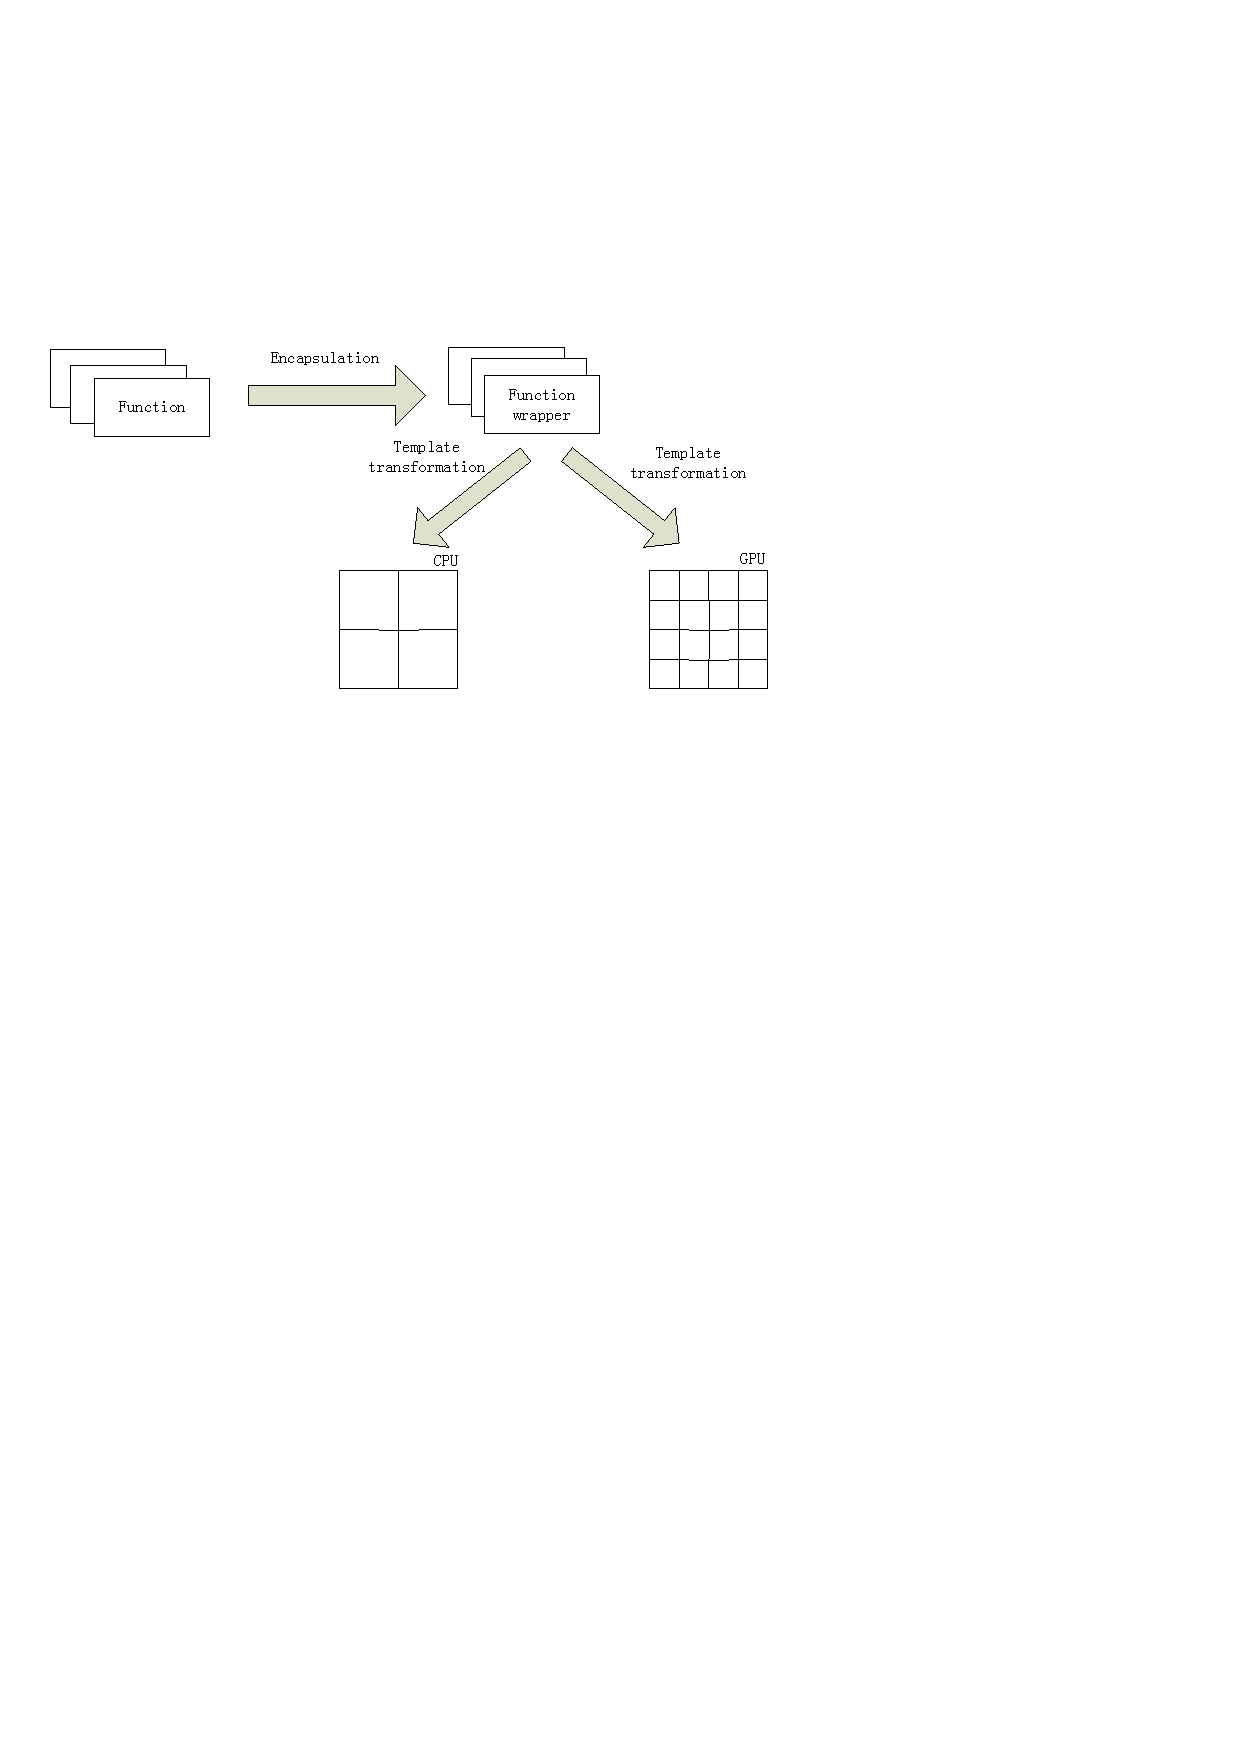
\includegraphics[width=3.3in, height=4.0in]{../overview}
\caption{Overview of template-based programming model: Programmers
write side-effect free functions in C/C++, and then encapsulate them in
template classes. Such a template encapsulates the computing function and can be 
automatically transformed into a
group of subtasks by TF classes based on appropriate parallel patterns. Finally,
subtasks directly run on physical multicores.}
\label{fig:overview}
\end{figure}

We propose a template metaprogramming approach to support parallel programs
running on different multicore systems. \reffig{overview} gives an overview
of our approach: a side-effect free function is abstracted as a \emph{task}
and is wrapped in a template class. We provide template classes
to support different parallel patterns:

\begin{itemize}
\item \textbf{Hierarchy pattern.} A task is recursively divided into subtasks
and subtasks can execute on multiple cores in parallel.

\item \textbf{Pipeline pattern.} A task is divided into a series of processing
subtasks, where the output of a previous subtask is directly used as the input
of the next subtask and each subtask execute on a core.

\item \textbf{MapReduce pattern.} A task is divided into a map phase and a
reduce phase, where subtasks in each phase can execute in parallel on multiple
cores. The input of reduce phase is the output of the map phase.

\end{itemize}

The transformation for a task from sequential code to parallel equivalence is a
source-to-source conversion with C++ templates, which is enabled by a \emph{TF
class} (Section~\ref{sect:tf}).  The converted code calls
architecture-specific building block classes (Section~\ref{sect:bb}) so that
when compiled, a task can execute on
different multicore systems in parallel at run time. 

The rest of this section first describes three class types of our approach, i.e.,
TF, view, and building block classes. 
%(1) View class, a representation of underlying containers such as vector or matrix.
%(2) Building block class,
%provide basic executions of tasks on multicores (3) TF class, each one
%represents a parallel pattern. 

\subsection{TF Classes}
\label{sect:tf}

A \textit{TF class} (short name for \textit{TransFormation class}) is a template
class representing a parallel pattern that transforms a task to a group of
subtasks in isomorphism. In other words, the transformed task has the same interface
while owns a call graph inside to complete the original computation by a
group of subtasks. Specifically, the following two classes are used in this paper: 

\begin{itemize} 
\item \textbf{TF\_hierarchy}. This template class recursively divides a task into subtasks
until certain predicate is evaluated as true. %As Fig.~\ref{fig:mmexample} depicted,  we use
In fact, \code{TF\_hierarchy} can implement a programming model similar to Sequoia and
we use \code{TF\_hierarchy} to implement both hierarchy and MapReduce pattern.

\item \textbf{TF\_pipeline}. This template class synthesizes a call chain of an
arbitrary number of functions into a pipeline. This is a common pattern for
stream kernel programming model.
\end{itemize} 

\subsubsection{TF\_hierarchy}

\reffig{tf:code} illustrates the class definition of \code{TF\_hierarchy}. The
prime template (line 1 to 10) takes  user supplied \code{TASK}
class and a predicate class as parameters. Note the third parameter, the bool value,
is calculated from the predicate class at compile time, so programmers don't
use this parameter. 
The predicate class is similar to Merge~\cite{merge} and is used to generate
control flow for recursions. The main difference from Merge is that our predicate is a
\emph{metafunction} and is evaluated in place to obtain the bool value, which
depends on the two types, \code{TASK::ARG0} and \code{TASK::ARG1}
defined in the class \code{TASK}. Usually these two types are views (Section~\ref{sec:view})
with statically known sizes. When the third parameter is evaluated as false, the
prime template is used and \code{doit} function invokes recursive
\code{TASK:inner} function, which divides a task into subtasks.
On the other hand, when the third parameter is evaluated as true, the partial
specialization template (line 12 to 19) is used, where \code{doit} function
invokes \code{TASK::leaf} function (leaf node, no recursion).


\begin{figure}[hbt]
  \inputsrc{tf.cc}
  \caption{Pseudo-code of class \code{TF\_hierarchy}.}
  \label{fig:tf:code}
\end{figure}

\begin{figure}[hpt]
  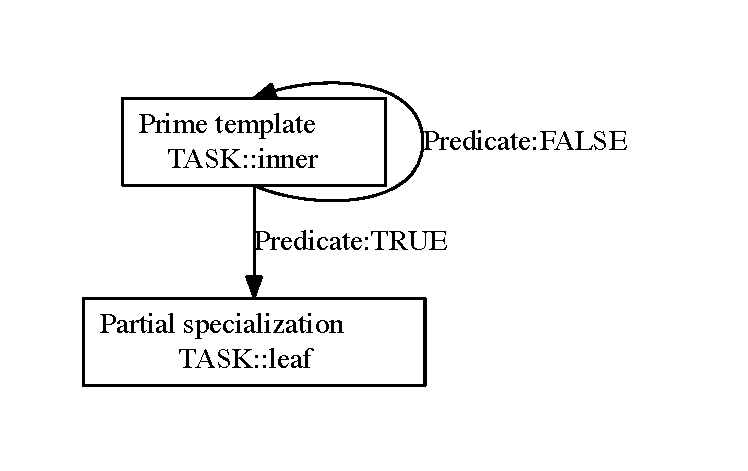
\includegraphics[width=3.0in]{../algo}
  \caption{Instantiation process of \code{TF\_hierarchy}. The predicate is a template
class, which is evaluated using \code{TASK}'s parameters.}
  \label{fig:hierarchy}
\end{figure}

The instantiation process of \code{TF\_hierarchy} is illustrated in \reffig{hierarchy}:
when predicate is false, the task is recursively divided into subtasks; when predicate
is true, the code (\code{TASK::leaf}) computes a subtask.

%A side-effect free function is referred to as \emph{task} in
%libvina. As a rule of thumb,
%nFIXME
\comment{In this paper, we consider a class of computation-intensive functions (or tasks) that are 
self-contained, i.e., external data references are limited and
calling graphs of them are simple. For these functions, it's possible to
decouple a task into a cluster of subtasks. These subtasks are identical
except for arguments and we can distribute subtasks on multicore to execute simultaneously. 
}

%We implement two TF classes in libvina though  it is not
%necessary to use TF classes to perform source transformations. We
%encourage to do so because it has engineering advantages, which reduces
%effects of system programmers.

\subsubsection{TF\_pipeline}
The \code{TF\_pipeline} class using variadic template~\cite{vartemp} is
illustrated in \reffig{pipeline:code}. \code{TF\_pipeline} supports an arbitrary
number of functions chaining together and the only limitation is the maximal
level of template recursions of a compiler.

%For C++ compilers don't support variadic template, there
%are workarounds to achieve the same effect, but quite
%tedious.\footnote{zhangsq ask me to cite. I implemented the
 % workarounds myself, but i don't see it is necessary to show them here. too
 % details... --xliu 28. Nov}.

\begin{figure}[hbt]
  \inputsrc{pipeline.cc}
  \caption{Pseudo-code of class \code{TF\_pipeline}.}
  \label{fig:pipeline:code}
\end{figure}


\subsection{View Classes}
\label{sec:view}

A \emph{View} is a class representing a subset of container's data. For example,
a matrix type could have views that contain a subset of elements of a matrix.
There are two kinds of views, \code{ReadView} and \code{WriteView}.
A \code{ReadView} is read-only, while a \code{WriteView} allows write operations on its data
(by providing interfaces to write). 

To ensure thread safety, \code{ReadViewMT} and \code{WriteViewMT} are
defined. For these two types, each object contains a signal that is copied across multiple
threads. All operations of \code{ReadViewMT} or \code{WriteViewMT} are blocked until
other threads signal the current thread.

\reffig{view} depicts the relationship of views. A concrete line means that
a type cast from a source node to a destination node is legal, i.e., an implicit
conversion in C++.  A dashed line means a source node can generate objects of
the type of the destination node. Labels on the dashed line signify how
signals are created or copied.
Shadow region is another thread's space.

%The only approach to communicate with other
%threads is through a special kind of view called \emph{ViewMT}.  

The design of view class serves two purposes. 1) The classes are type-safe.
Because template instantiation is invisible for programmers, our
source transformations by templates may introduce subtle errors. We
expect compilers complain explicitly when unintentional
transformations happen. For example, when a \code{ReadView} is accidently used
for writes, the compiler will complain for errors. 2) View classes hide architecture specifics. %communication details. 
Implementations have choices to optimize data movement according to
architectures. Shared memory systems~\cite{larrabee} and communication-exposed
multicores~\cite{cellbe, imagine} usually have different strategies to perform
the operations. In fact, our implementation of for CPU and GPU are different (See
Section~\ref{sec:details}).

\begin{figure}
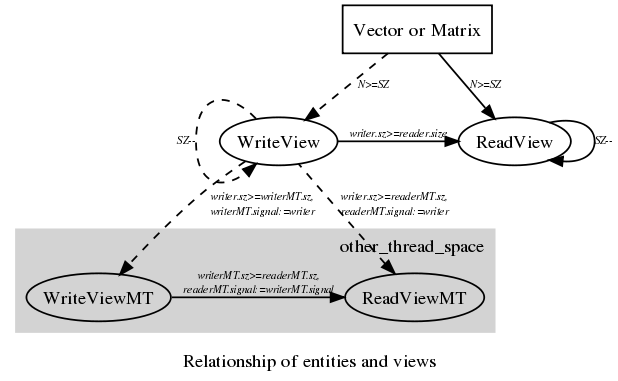
\includegraphics[width=3.6in, height=2.5in]{../relationship_views}
\caption{The relationship of view classes. A concrete line represents a valid
   type cast, while a dashed line represents a source node can generate objects
of the type pointed to. Labels specify how signals are created or copied
across views.}
\label{fig:view}
\end{figure}


\subsection{Building Block Classes}
\label{sect:bb}

\begin{table}[hbt]
\caption{Building block classes in libvina}
\begin{tabular}{|c|l|l|}
\hline
Name& Semantics& Usage Example\\
\hline
\textbf{par$<$T, K, F$>$}& Iterate function \textit{F} \textit{K} times &par$<$\_tail, 4, F$>$\\ 
                         &in parallel, implicit barrier                 &::apply();\\                
\hline
\textbf{seq$<$T, K, F$>$}& Iterate function \textit{F} \textit{K} times&seq$<$\_tail, 5, F$>$\\
                         &                                             &::apply();\\
\hline
\textbf{reduce$<$K, F$>$}&Reduce \textit{K} values using &reduce$<$8, F$>$\\
&function
\textit{F}&::apply(values)\\
\hline
\textbf{mt::thread$<$F$>$}&Spawn a thread to execute  & mt::thread$<$F$>$\\
                          &function \textit{F}        & ::apply();\\
%\textbf{do\_}&loop until predicate is evaluated true.& 
\hline
\end{tabular}\label{tbl:bb}
\end{table}

A building block class is a high-level abstraction of executions that
hide architecture-specific details. Programmers can use building blocks to
execute tasks on different multicore platforms.
\reftable{bb} lists building blocks in libvina. For tasks that can
executed in a SPMD (Single-Program-Multiple-Data) fashion, \code{par} class spawns
multiple threads to execute iterations in parallel. \code{seq} class 
executes iterations in order. Parameter $T$ in \code{par} or \code{seq} could be nested
\code{par}, nested \code{seq}, or \code{\_tail} (meaning no further nesting).
For instance, we can write the following statement 

%However, if it is
%not the case, we have to deal with dependences carefully using \code{seq} and \code{reduce}. 
%Like traditional programming languages, our
%building blocks of iterations support nesting definition. In addition, both \textit{seq} and
%\textit{par} are interoperable. 

\begin{lstlisting}
seq<par<_tail, 4>, 3, F>::apply();
\end{lstlisting}
to build to a two-level loop, and the nested loop are executed in
parallel. The equivalent OpenMP code is:
\begin{lstlisting}
F f;
int i, j;
for (i=0; i<3; ++i)
{
  #pragma omp parallel for private(j)
  for (j=0; j<4; ++j){ 
    f(i, j);
  }//implicit barrier
}
\end{lstlisting}

%The first template parameter $T$ of iterations is used to support nest. It could be
%either a par or a seq. Special classes \code{par\_tail} and \code{seq\_tail} are
%symbols to indicate the end of nest.

The \code{reduce} class supports the ``reduce'' pattern in MapReduce style tasks.
Specifically, a given function $F$ is used to reduce $K$ input values and the
final result is stored in the first value. Note that many of the $K-1$ times
reduce operations are executed in parallel using multiple threads.

Finally, \code{mt::thread} class provides a thread interface for programmers to
dynamically spawn a new thread to execute a function.

%can exploit it to bind thread directly (\textit{e.g.} line 19 of List 2)
%or develop other customized building blocks.



%programming model
\comment{
We use template metaprogramming to implement a parallel programming model.
Essentially, our approach utilizes C++ template mechanism to
perform source-to-source transformations for multicores. Side-effect
free functions are abstracted as \emph{tasks}. A task is
wrapped in the form of template class, named \emph{function
  wrapper}.  A \emph{TF class} is a template class, which
is capable of transforming a task into a group of subtasks based on
a parallel pattern. Tasks
apply TF classes according to their appropriate
parallel patterns. This process is called ast \emph{adaption}. 
Finally, we use \emph{building block classes} to define executions of tasks
on specific architectures. Both TF classes and building
blocks are organized as a library --
\textbf{libvina}.}



\section{Libvina: A template library}\label{sec:lib}
We implement a prototype template library, libvina,  to demonstrate
our approach. Libvina consists of 3 components: (1) View class, a representation of underlying containers such as vector or matrix. (2) Building block class,
provide basic executions of tasks on multicores (3) TF class, each one
represents a parallel pattern. 

\subsection{View class}
To leverage static information, libvina need to
associate template parameters with ADTs' parameters. For example, 
Matrix class cantains 3 template paramters: type, the number of
row, the number of column. A definition of Matrix is at line 26 of
List 1. A \emph{View} is a class representing the subset of containers' data. There
are two kinds of views: ReadView and WriteView. Variants like
ViewMTs serve for multithreaded programs. 
A ReadView is read-only. A WriteView has interfaces to write  as
well. ViewMTs contains signals, which are copied across multiple
threads. All operations of ViewMTs are blocking until signals are sent
by other views.

Fig.~\ref{fig:view} depicts relationship of views in
libvina. Concrete lines represent implicit conversion in C++, while
dashed lines are explicit function calls to complete conversion. Text
in edges are constraints for conversions. Line 30$\sim$32 of
List 1 generate subviews by calling functions. Shadow region is
another thread space.
%The only approach to communicate with other
%threads is through a special kind of view called \emph{ViewMT}.  

The design of view class has two purposes. 1) The classes are type-safed.
Because template instantiation is not visible for programmers, our
source transformations by templates could introduce subtle errors. We
expect compilers complain explicitly when unintentional
transformations happen. 2) View classes hide communication details. 
Implementations have choice to optimize data movement according to
architectures. Shared memory systems~\cite{larrabee} and communication-exposed multicores~\cite{cellbe, imagine} usually have different strategies to perform
the operations.

\begin{figure}
%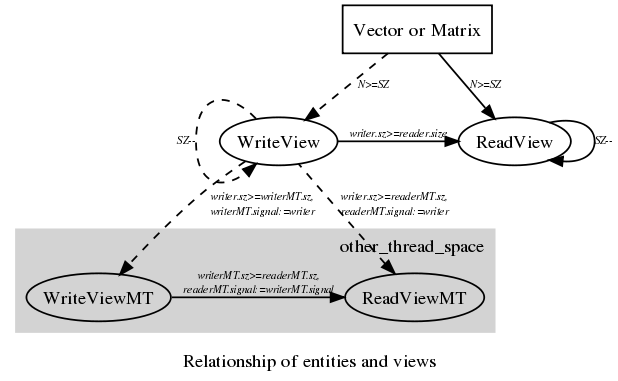
\includegraphics[width=3.6in,height=3.0in]{../relationship_views}
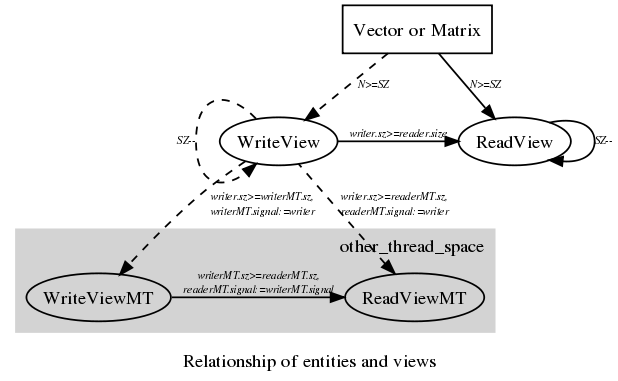
\includegraphics[width=3.6in, height=2.5in]{../relationship_views}
\caption{View classes in libvina: A view represents subset of
  underlying constrainers. A ReadView is read-only. A WriteView
  can write back as well. Edges are  conversions. A concrete line is implicit conversion from head to
  tail, while a dashed line represents a conversion needs explicit function
  call. ViewMTs are used for multithreaded programs. A
  signal in ViewMT is a handler of dependence.}\label{fig:view}
\end{figure}

\subsection{Buiding block class}
A building block class is a high-level abstraction of execution. Programmers
utilize building blocks to execute tasks on multicores.
Table.~\ref{tbl:bb} lists building blocks we implement in libvina. To parallelize programs, we expect most tasks are
executed in SPMD (Single-Program-Multiple-Data). However, if it is
not the case, we have to deal with dependences carefully using \textit{seq} and \textit{reduce}. At last, we
provide thread interface using mt::thread class. Programmers can
exploit it to bind thread directly (\textit{e.g.} line 19 of List 2)
or develop other customized building blocks.

Like traditional programming languages, our
building blocks of iterations support nesting definition. In addition, both \textit{seq} and
\textit{par} are interoperable. \textit{i.e.} we can write statement like 
\begin{lstlisting}
seq<par<par_tail, 4>, 3, F>::apply();
\end{lstlisting}
to build to a level-2 loop, and the nested loop are executed in
parallel. Its equivalence in OpenMP is as follows:
\begin{lstlisting}
F f;
int i, j;
for (i=0; i<3; ++i)
{
  #pragma omp parallel private(j)
  for (j=0; j<4; ++j) 
    f(i, j);
}//implicit barrier
\end{lstlisting}
The first template parameter T  of iterations is used to support nest. It could be
either a par or a seq. Special classes \textit{par\_tail} and \textit{seq\_tail} are
symbols to indicate the end of nest.

\begin{table}[hbt]
\caption{Build blocks in libvina}
\begin{tabular}{|c|l|l|}
\hline
Name& Semantics& Example\\
\hline
\textbf{seq$<$T, K, F$>$}& Iterate function \textit{F} \textit{K} times&seq$<$seq\_tail, 5, F$>$\\
&&::apply();\\
\hline
\textbf{par$<$T, K, F$>$}& Iterate function \textit{F} \textit{K} times
&par$<$par\_tail, 4, F$>$\\ 
&in parallel, implicit barrier&::apply();\\                
\hline
\textbf{reduce$<$K, F$>$}&Reduce \textit{K} values using &reduce$<$8, F$>$\\
&function
\textit{F}&::apply(values)\\
\hline
\textbf{mt::thread$<$F$>$}&Eexecute function \textit{F} &mt::thread$<$F$>$\\
&in a thread&::apply();\\
%\textbf{do\_}&loop until predicate is evaluated true.& 
\hline
\end{tabular}\label{tbl:bb}
\end{table}

\subsection{TF class}
TF class is the short form of \textit{TRansformation class}.  A
side-effect free function is referred to as
\emph{task} in libvina. As a rule of thumb,
computation-intensive functions are usually
self-contained, \textit{i.e.} external data references are limited and
calling graphs of them are simple. Therefore, it's possible to
decouple a task into a cluster of subtasks. The subtasks may be identical
except for arguments and we can distribute subtasks on multicore to execute simultaneously.  Another approach is to divide a complicated task into finer stages
and run in pipeline manner to respect data locality and bandwidth. Two
examples mentioned before follow the two patterns respectively. A
\textit{TF class} is a template class representing a parallel pattern which
transforms a task to a group of subtasks in
isomorphism. \textit{i.e.} the transformed task has the same interface
while owns a call graph inside to complete the original computation by a
group of subtasks. 

We implement two TF classes in libvina though,  it is not
necessary to use TF classes to perform source transformations. We
encourage to do so because it has engineering advantages, which reduces
effects of system programmers.

\begin{itemize} 
\item TF\_hierarchy It will recursively divide task into subtasks until
  predicate is evaluated as true. As Fig.~\ref{fig:mmexample} depicted,  we use
  TF\_hierarchy to implement programming model like Sequoia.

\item TF\_pipeline Inputing an arbirary number of functions, the template
  class can synthesize a call chain. This is a common pattern for
  stream/kernel programming model.
\end{itemize} 

\section{Adaption for Libvina}\label{sec:adaption}
Programmers who apply our approach need to customize their source code
to utilize libvina. Technically speaking, we provide a group of \emph{concepts}
in libvina to support transformations and expect programmrs to \textit{model} our template classes~\cite{tempmetaprog}. 

\subsection{Function Wrapper}
Function wrapper is an idiom in libvina. Our approach needs to manipulate
template functions according to their template arguments. However, a
template function is unaddressable until it is
instantiated. Thus programmers have to bind their template functions
to entries of classes.  Either static function or call operator
fuctions is approachable though,
there is tradeoff to consider. Static function need to predefine naming convention. 
\textit{e.g.} TF\_hierarchy use names \textit{inner} and
\textit{leaf} to call back. Call operator has unique form to invoke, so we leave it
as user interface, at expense of runtime
cost\footnote{C++ does not allow overload call operator using static
  function, therefore we have to generate a object to call it.}. Line 14
of List 1 is the case.

%Another restrict of function is that our
%template can only handle fixed form of function. \textit{i.e.} the
%function signature is triple form\footnote{function form: void (ARG0, ARG1,
% RESULT).We expect template alias in C++0x can releave this
%  retrict. } and parameter passing semantics is CBVR~\cite{dragonbook}.

\subsection{Adaption for TF\_hierarchy}
Line 6$\sim$10 of List 1 is adaption for TF\_hierarchy. Line 10
defines the type of task for SGEMM. It is used as
the template parameter TASK for TF\_hierarchy class. PRED template
parameter at line 11 is a predicate and TF\_hierarchy class will
evaluate it using ARG0 and ARG1. Line 18 calls customized TF class after dividing
task. According to template argument, TF class determines whether
reenter the entry inner at line 22 or terminate at leaf at
line 45. Function leaf performs computation. Fig.~\ref{fig:hierarchy} illustrates
instantiation process of TF\_hierarchy and Fig.~\ref{fig:mmexample} is
execution after transformation. The figure depicts the case K is 2.

\begin{figure}[hpt]
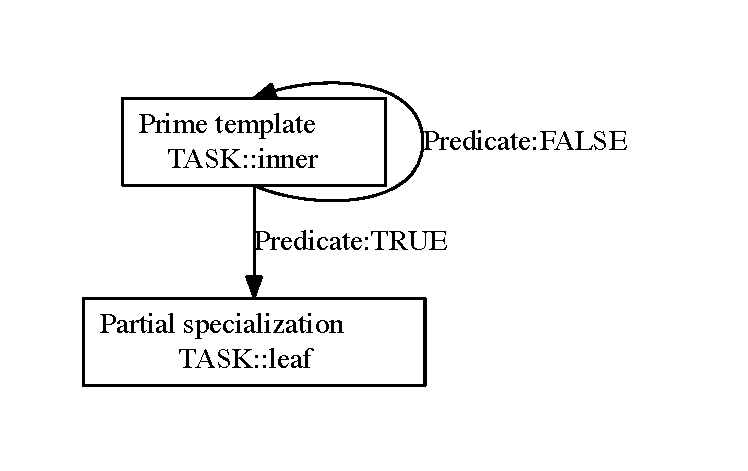
\includegraphics[width=3.5in]{../algo}
\caption{Instantiation process of TF\_hierarchy: The predicate is a template
class, which is evaluted using TASK' parameters.}\label{fig:hierarchy}
\end{figure}
%for sequoia's programming mode: 
%define recursive rules 
% for stream 's programming model:

\subsection{Adaption for TF\_pipeline}
To leverage TF\_pipeline, programmers have to provide a full
specialization template class for it. This is because TF\_pipeline
only synthesizes functions and executes them in order. It does not
know how to process the output. A full specialization of TF\_pipeline very defines
this behavior and is called at last. For \textit{langpipe} example,
line 2$\sim$21 is the case. Static entry at line 13 serves TF\_pipeline class. We spawn a thread to handle with the output of
precious last stage. Line 24$\sim$31 is a usage of TF\_pipeline with 4
standalone functions. All the stages including our customized one are
threads. It is noteworthy that each immediate stage \textit{e.g.}
\textit{translate$<$Frn2Spn$>$} has to follow type interfaces and
define dependences. In \textit{lang\_pipe} case, we utilize our ViewMT
despicted in Fig.~\ref{fig:view}. Asynchronous signals in ViewMTs provoke waiting
stages and are used to mimic data-flow diagram. Fig.~\ref{fig:viewmt} illustrates the scenario contains three
threads.

\begin{figure}[tp]
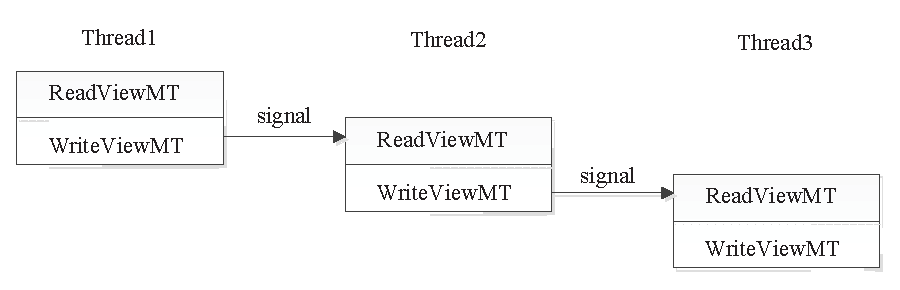
\includegraphics[width=3.1in]{../viewmt}
\caption{Pipeline process using ViewMTs: Access of a ViewMT is
  blocking until it is signaled. A stage sets its signal of WriteViewMT
after processing.}\label{fig:viewmt}
\end{figure}

%end of section.
\section{Implementation}
\label{sec:details}

We implement all the functionalities described before using C++
template metaprogramming techniques.
The main idea is to utilize
template specialization and recursion to manage control flow at
compile time. Besides template mechanism, other C++ high-level
abstractions play an important role in our approach.
Function objects and bind mechanism are commonly employed to postpone computation
at proper places with proper environment~\cite{moderncpp}.
%In order to utilize nested building blocks,
%lambda expression can generate closure objects in a concise
%form, e.g., line 24$\sim$37 of \reffig{sgemm}.

We implemented libvina in ISO C++ following the new C++ standard (i.e., C++0x\cite{c++0x}),
because C++0x adds many language features to ease metaprogramming~\footnote{When
we conduct this work, C++0x standard is close to finish. Implementing C++0x is a work in
progress for many compilers, including GCC and Intel compiler.}. Compilers
without C++0x support need some workarounds, which are also implemented in our
library.
%Theoretically, any standard-compliant C++ compiler
%should process our library without trouble. 

Implementation of building blocks is straightforward. We use recursive calls
to support nesting patterns. \code{seq} and \code{par} are interoperable
because we chose properly nested classes before calling function \code{apply}.
%Note that building blocks do not know the nesting levels during the execution. To solve this
%problem, each function object or closure object is decorated with a loop-variable counter.
%The handlers take responsibility for calculating loop variables in
%normalized form. It is only desirable for nested loop forms,
%\textit{e.g.} line 41 of List 1.
Because some callable objects in C++ such as closure object
do not provide default constructors, we pass their
references in those cases. 
%Consequently, some call sites of building blocks are different from \reftable{bb}.

For CPU, building blocks are implemented by embedding OpenMP directives. On GPU, we bind
building block classes to functions of OpenCL~\cite{opencl}, an open standard API
for heterogeneous multicores. For instance, we use OpenCL's \code{NDRangeKernel} function
to implement \code{par} template class. The \code{mt::thread} is implemented using pthread.
For the signal mechanism among views, conditional variables of pthread are used
for CPU and events are employed for GPU.

%Because GPUs momory model is different from CPU memory
%hierarchy, applying source transformation of TF\_hierarchy makes
%little sense, so we directly use building
%blocks to translate iterations into OpenCL's NDRangeKernel function. 

\section{Experiment}\label{sec:eval}
\subsection{Methodology}\label{sectn:method}
%compiler and libs
We implement our library in ISO
C++. Theoretically, any standard-compliant C++ compiler
should process our classes without trouble. New C++ standard (a.k.a C++0x\cite{c++0x}) adds many language features to ease metaprogramming\footnote{When we
  conducted this work, C++0x was close to finish. Iimplementing C++0x
  were in progress for many compilers}. Compilers
without C++0x support need some workarounds to pass compilation
though, they do not hurt expressiveness.We developed the library and
tested using GCC 4.5 beta.  The
first implementation of OpenCL was shipped by Mac OSX 10.6. The GPU performance is collected on that platform.

% Consider the trend of C++,
%development of template library like libvina should become easier
%and smoother in the future.  

A couple of algorithms are evaluated for our template approach.  They
are typical in image processing and scientific fields. In
addition, we implement a pseudo language translation program to
illustrate pipeline processing. The programs in experiments are listed
as follows:

\begin{itemize}
\item[\textit{saxpy}] Procedure in BLAS level 1. A scalar multiplies to a single precision vector, which contains 32 million elements.
\item[\textit{sgemm}] Procedure in BLAS level 3. Two 4096*4096 dense matrices multiply.
\item[\textit{dotprod}] Two vectors perform dot production. Each vector
  comprises 32 million elements.
\item[\textit{conv2d}] 2-Dimensional convolution operation on image.  The Image
  is 4094*4096 black-white format. Pixel is normalized as a single
  float ranging from 0.0 to 1.0.
\item[\textit{langpipe}] Pseudo-Multi-language translation. A word is translated from one language A to language B, and then another function will translate it from language B to language C, etc.
\end{itemize}

Two multicore platforms are used to conduct experiments. The hardware
platforms are summed up in Table.~\ref{tbl:mach}

\begin{table}[hbt]
\caption{Experimental platforms}\label{tbl:mach}
\begin{center}
\begin{tabular}{|l|l|l|l|l|r|}
\hline
\textbf{name}&\textbf{type}&\textbf{processors}&\textbf{memory}&\textbf{OS}\\
\hline
harpertown&SMP &x86 quad-core  &4G&Linux Fedora\\
                  &  server &   
2-way  2.0Ghz & &kernel 2.6.30\\
\hline
macbookpro&laptop &x86 dual-core &2G&Mac OSX\\
                    &           & 2.63Ghz         &  &Snowleopard\\
                   &           &GPU 9400m    &256M & \\
                    &           & 1.1Ghz   & &\\
\hline
\end{tabular} 
\end{center}
\end{table}
On harpertown, we link Intel Math kernels to perform BLAS procedures
except for conv2d. On macbookpro, we implemented all the algorithms on
our own. For CPU platform, we link libSPMD thread library to
perform computation. The library binds CPUs for each SPMD
thread and switch to realtime scheduler on Linux.  This configuration
helps eliminate the impact of OS scheduler and other processes in the
system.

\subsection{Evaluation}
\subsubsection{Speedup of Hierarchical transformation on CPU}
\begin{figure}
\includegraphics{speedupx86.0}
\caption{Speedup on Harpertown}\label{fig:spdx86}
\end{figure}

Fig.~\ref{fig:spdx86} shows the speedup on harpertown. The blade
server contains two quad-core Xeon
processors. We experiment hierarchical transformation for
algorithms. All predicates are set to cater to CPU's last level cache(LLC).

We obverse good performance scalability for programs
\textit{conv2d} and \textit{sgemm}. \textit{conv2d} does not have any dependences
and it can obtain about 7.3 times speedup in our experiments. \textit{sgemm}
needs an extra reduction for each division operation. The final
speedup is about 6.3 times when all the cores are available. Note that we
observe almost two-fold speedup from sequence to dual core case. But the speedup degrates to 3.3 times when executionu
environment changes to 4-core. Harpertown consists of 2-way quad-core processors,  Linux
can not guarantee that 4 subtasks are distributed in a physical
processor. Therefore, the cost of memory accesses and synchronization
increases from 2-core to 4-core.

\textit{dotprod} and \textit{saxpy} reveal low speedup because non-computation-intensive
programs are subject to memory bandwidth.  In average, \textit{saxpy} needs one load and one 
store for every two operations. \textit{dotprod} has similar
situation. They quickly saturate memory bandwidth for SMP system and
therefore perform badly. Even though we fully parallelize those
algorithms by our template library. 

\subsubsection{Speedup of  SPMD transformation on GPU}
\begin{figure}
\includegraphics{speedupgpu.0}
\caption{Speedup Comparing GPU with CPU}\label{fig:spdgpu}
\end{figure}

Fig.~\ref{fig:spdgpu} shows SPMD transformation results for GPU on
macbookpro. GPU's memory model has significantly different from
GPU. Because TF\_hierarchy makes little sense for GPU, we directly use building
block par to translate iterations into OpenCL's NDRangeKernel
function. Programs running on host CPU  in sequence are set as
baseline. Embedded GPU on motherboard contains 2
SMs\footnote{Streaming Multiprocessor, each SM consists of 8 scalar processors(SP)}.
Porting from CPU to GPU, developers only need a couple of lines to change
templates while keeping algorithms same \footnote{
Because GPU code needs special qualifiers, we did modify kernel
functions a little manually.  Algorithms are kept except for sgemm. It is not easy
 to work out sgemm for a laptop, so we added blocking and SIMD
 instruments for CPU.}. As figure depicted,  computation-intensive programs
\textit{sgemm} and \textit{conv2d} still maintain their speedups. 4.5 to 5 times
performance boost is achieved for them by migrating to GPU.
In addition, we observe about 2 times performance boost for
\textit{saxpy}. Nvidia GPUs execute
threads in group of warp (32 threads) on hardware and it is
possible to coalesce memory accesses if warps satisfy
specific access patterns. Memory coalescence mitigates bandwidth issue
occurred on CPU counterpart. Because our program of \textit{dotprod} has fixed
step to access memory which does not fit any patterns, we can not
obtain hardware optimization without tweaking the algorithm.

\subsubsection{Comparison between different multicores}
\begin{table}[hbt]
\caption{Comparison of sgemm on CPU and GPU}\label{tbl:sgemm}
\begin{tabular}{|l|r|r|r|}
\hline
& baseline& CPU & GPU\\
\hline
\textbf{Cores} &1 x86(penryn)& 8 x86(harpertown)& 2 SMs\\
\hline
\textbf{Gflops}& 2.64 &95.6&  12.0\\
\hline
\textbf{Effectiveness}&12.6\%& 74.9\%&68.2\%\\
\hline
\textbf{Lines of function}&63&unknown&21\\
\hline
\end{tabular}
\end{table}

Table.~\ref{tbl:sgemm} details \textit{sgemm} execution on CPU and GPU. Dense matrix
multiplication is one of  typical programs which have
intensive computation. Problems with this characteristic are the most
attractive candidates to apply our template-based approach.
Our template library transforms the \textit{sgemm} for both CPU and 
GPU. We choose sequential execution on macbookpro's CPU as
baseline. After mapping the algorithm to GPU, we directly obtains over
4.5 times speedup comparing with host CPU. Theoretically,  Intel Core
2 processor can issue 2 SSE instructions per cycle,  therefore, the
peak float performance is 21 Gflops on host CPU. We obtain 2.64 Gflops which
effectiveness is only 12.6\% even we employ quite complicated
implementation. On the other side, 12 Gflops is observed on GPU whose
maximal performance is roughly 17.6 Gflops.\footnote{$17.6Gflops = 1.1Ghz * 2(SM) *
  8(SP)$. nVidia declared their GPUs can perform a mad(multiply-add
  op) per cycle  for users who concern performance over precision. However, we can
  not observe mad hints bring any performance improvement in OpenCL. }
Although both column 2 and column 4 implement SIMD algorithm for
\textit{sgemm}, GPU's version is obviously easier and effective. It is
due to the dynamic SIMD and thread management from GPU
hardware~\cite{Fatahalian08} can significantly ease vector programming. Programmer can
implement algorithm in plain C and then replies on template
transformation for GPU.  Adapting to GPU only need tens of lines code
efforts. Like GPU template, we apply building blocks directly to parallelize \textit{sgemm} procedure for CPU. We observe 95.6 
Gflops and about 75\% effectiveness on harpertown server.

\subsubsection{Pipeline Transformation for CPU}
\begin{figure}[htp]
\includegraphics{pipeline.0}
\caption{Pipeline Processing for Psuedo Language Translation}\label{fig:pipe}
\end{figure}

Fig.~\ref{fig:pipe} demonstrates pipeline processing using our
template library. As described before, \textit{langpipe} simulates a
multilingual scenario. We apply template TF\_pipeline listed in
List. 2. In our case, the program consists of 4 stages,
which can transitively translate English to Chinese\footnote{follow the 
  route: English  $\to$ French $\to$ Spanish $\to$ Italian $\to$
  Chinese}. Only the preceding stages complete, it can proceed with
the next stages. The executing scenario is similar to Fig.~\ref{fig:viewmt}. We use bogus loop to consume $t \  \mu s$ on CPU. For each $t$, we iterate 500
times and then calculate the average consumptive time on harpertown. For
grained-granularity cases (20$\mu s$, 50$\mu s$, 100$\mu s$), we can obtain ideal
effectiveness in pipelining when 4 cores are exposed to the system.
\textit{i.e.} our program can roughly output one instance every $t\  \mu
s$. The speedup is easy to maintain when granularity is big. 100 $\mu s$ case ends up 54 $\mu s$ for each instance for 8 cores. 50  $\mu s$ case
bumps at 5 cores and then improves slowly along core increment. 20
$\mu s$ case also holds the trend of first two cases. 5 $\mu s$ case is
particular. We can not observe ideal pipelining until all 8
cores are available.  Our Linux kernel scheduler's granularity is 80
$\mu s$ in default. We think that the very fine granular tasks contend
CPU resources in out of the order. The runtime behavior presumably
incurs extra overhead. Many cores scenario helps alleviate the
situation and render regular pipeline processing.


\section{Related work}\label{sec:related}
%As mentioned before, it is desirable to extend conventional
%programming languages to reflects new hardwares. Researches in the field have two major directions:
To meet challenges of multicore, approaches based on existing
programming languages can be broadly categorized into two classes: A) library-based approaches, which
provide libraries to support parallel programs, and B) Compiler-based
approaches, which extend new language grammars or constructs for parallelism.

Library-based approaches extend programming languages
by well-developed libraries. Because both development and adaption of
the libraries are based on original language infrastructures, the
workload of programmers is relatively reduced. Many systems provide
such libraries to expose interfaces for parallel programs such as
Pthread (POSIX Thread), MPI (Message Passing Interface), and
OpenCL~\cite{opencl}. However, system-level libraries usually rely on 
their underlying platforms. Abstractions
of those libraries are usually far away from expressing parallelism
naturally, and it is difficult to
port programs from one library to another. Our library is a
metaprogramming library for source transformations. It contains template classes which abstract high-level parallel patterns
and executions, instead of the interfaces of system primitives or
resources. On the other side, system-level libraries, developing high-level
library to support parallelism and concurrency is also a hot topic in
programming language field~\cite{javacon, wincon}. C++ community intends to
achieve the target while bearing generic programming in mind.  TBB~\cite{tbb} has a plenty of
containers and building blocks to support loop-parallelism and
task-level parallelism.  Inspired by TBB's approach, we achieve the
same effects in static domain. We aim at using static information
to tailor to different multicore architectures. Besides, the template-based
approach we proposed is orthogonal to runtime parallel libraries. We
only exploit parallelism which can be resolved by compilers,
programmers feel free to employ other runtime approaches for further improvement.

%\textit{e.g.} Pthread is a
%\textit{de facto} standard interface of multithread for
%POSIX-compatible systems. 
%Furthermore, the implementation of thread on hardware is
%undefined in the standard, so it can not guarantee performance or even
%correctness on some architectures \cite{Boehm05}.

%Entities including partitioner and
%scheduler in TBB are created at run time. In that case, key data
%structures have to be thread-safe. Although TBB exploits task
%parallelism or other sophisticated concurrency on general purpose
%processors, the runtime overhead is relative high in data parallel
%programs, especially in the scenario that many lightweight threads are
%executing by hardware. 


%% MPI
%Another dominant parallel library is MPI in supercomputing community. It based on message-passing mechanism and SPMD model to execute parallel program. The difficulties of developing MPI programs are as notorious as pthread counterpart for programmers without sufficent training of parallel programming. 
%%

%OpenMP ~\cite{openmp} is designed for shared memory and has been shipped in almost every C/Fortran
%compilers.
%OpenMP can only perform Fork-Join parallel model.
%Source-to-Source transformation for optimization was reported by~\cite{Loveman77}, whose granularity of transformation  is
%statement.  Most of works have been merge in forms of IR in
%modern compilers. New source-to-source transformation compilers focus
%on function. 
%The run-time is usually provides in the form of dynamic link library.
%Although it is simple and
%portable, the performance is not optimal in most cases. Moreover, a
%handful of directives in OpenMP leave little room for further improving
%performance or scaling up to larger systems. Hybrid OpenMP with MPI is
%possible though, difficulties surge. 

In contrast, compiler-based approaches attempt to revise
programming languages per se. They add annotations or language constructs to
support parallel programs. Consequently, programmers
can describe parallel algorithms directly without caring about low-level executions.
OpenMP~\cite{openmp} compilers transform sequential code blocks into
multi-threaded equivalences according to directives. Although OpenMP
is \textit{de facto} standard for shared memory systems, it does not
support heterogeneous multicores. In order to achieve portability for
parallel programs, sequoia~\cite{sequoia, sequoia-compiler} transforms a \textit{task} into a cluster of
\emph{variants}, and uses Parallel Memory Hierarchy (PMH)
model~\cite{pmh} to map variants on physical architectures.
We derive the same idea from sequoia by transforming and mapping tasks
at compile time. Merge~\cite{merge} is a dynamic map/reduce programming
framework for heterogeneous multicores. It relies on the hierarchical division of tasks and predicate-based
dispatch system to assign tasks on matched targets at runtime. An obvious shortcoming of compiler-based approaches is that each
approach can only support one kind of parallel patterns. 

We intend to fuse the advantages of library-based approaches and
compiler-based approaches. Our approach performs source-to-source
transformations for different multicores by C++ template libraries. We
demonstrate that template metaprogramming is powerful enough to
implement multiple programming models.


%We think it is this process hardwires fixed parallel patterns into the
%compilers. Therefore, we explore the powerness of metaprogramming to
%transform sources for parallelism, which
%can support mulitple parallel programming models while maintain
%portability for multicores.

%First of all, it targets execution
%environment as a tree of machines, which an individual machine owns
%its storage and computation unit. Second, Target machine
%is described in XML files. \cite{sequoia} reports that Sequoia can transform programs
%for CellBE, cluster while keeping competitive performance. That
%is at expense of implementing one compiler for each platforms.
%The primary drawback of Sequoia is that its language constructs can not cover common
%parallel patterns such as pipeline or task queue. Methods mentioned before all need non-trivial efforts to
%modify compilers. As discussed in \cite{sequoia}, the authors of the Sequoia were
%still not clear whether the minimal set of primitives they provided provides can
%sufficiently express dynamic applications. We doubt if it is worthwhile to
%invest a compiler given the fact that template library can also
%achieve the same functionalities.

%end of section.
\section{Discussion and Future work}\label{sec:con}
%The silicon industry has chosen multicore as new
%direction. However, diverging multicore architectures enlarge the gap between algorithm-centric programmers and
%computer system developers.  Conventional C/C++ programming language
%can not reflect hardware.  Existing ad-hoc techniques
%or platform-dependent programming language pose issues of generality
%and portability. 
%Source-to-source transformation can meet the challenge
%and help tailor programs to specific multicore architectures.

%Not only the more processor cores but also
%elaborated memory hierarchy and exposed communication are adopted by
%new multicore architectures. More worse, 

We present a template metaprogramming approach to perform source-to-source
transformations for programs with rich information. All functionalities
are achieved within ISO C++ and organized as template library. The
library is flexible enough to
apply more than one parallel
pattern and execution model. In addition, programmers can extend library to
facilitate appropriate parallel patterns or new architectural
features because template metaprogramming is
intimate for C++ developers.  Experiments show
that our template approach can transform algorithms into SPMD threads
with competitive performance. These transformations are available for
both CPU and GPU, while the cost of migration is manageable. Besides, we
can apply hierarchical division for programs on CPU. We also
transform a group of standalone functions into a
pipeline using our template library. It demonstrates that template
metaprogramming is powerful enough to support more than one way to
parallelize for multicore.

%Our programming model bridges algorithm experts and diverging multcore
%architectures. Domain-specific experts focus on algorithms in form of
%conventional programming languages. They wrap functions to template
%classes and then pass them to \emph{TF class} as template parameter. Template
%mechniasm takes responisbility to transform source code according to
%their targets.

%Streaming is an important computation model for innovative
%multicore architectures~\cite{imagine, cellbe, larrabee, cuda}. We partially exploit GPU functionality in this
%paper, however, the transformations for GPU are quite
%straightforward.  It is still unclear how many efforts need to
%pay for a full-blown template library, which supports
%streaming computation.

% Libvina can only deal with regular
%data. Future work on view class  will concentrate on supporting
%general operations like gather and scatter etc.  
On CPU, source-to-source transformation should go on improving data
locality of programs. We plan to explore template approach to  generalize
blocking and tiling techniques.  It is also possible to re-structure
or prefetch data using template metaprograming accompanying with
runtime library.

Currently, kernel functions in GPU prohibit recursion. We believe that
it would be beneficial to introduce template recursion for
GPUs. In addition, it is attractive for us to explore source transformations for
strip-mined memory accesses in metaprogramming, becuse modern GPUs provide iprovide memory
coalescence to optimize memory.


General applications also contain a variety of static information to
optimize.The problem is that their memory footprints are irregular and
very hard to identify. It is desirable to explores new TF classes to facilitate
transforming source code close to target architectures using the static
information.

%\section*{Acknowledgements}

We would like to thank Weiliang Qian and Xiangyang Liu for helping me develop and test the codes.
We also thank Nicole Kwoh and Joanna Izabela Siebert for their technical discussions and proofreading.

This work is supported by the National High Technology Research and
Development Program (863 Program) of China (Grant No. 2006AA01Z172 and
2008AA01Z106), the National Natural Science Foundation of China (Grant
No. 60533040, 60725208 and 60773089), and Shanghai Pujiang Program
(Grant No. 07pj14049). This work is also partially supported by Hong Kong Polytehnic Univ under the grant
G-U513. 

\bibliographystyle{ieeetran}
\bibliography{libvina}

\end{document}
